\documentclass{article}
\usepackage{../AMadhava}
\rhead{MAT 533: Analysis II Notes}
\setcounter{secnumdepth}{0}
\usepackage{pgfplots,mathtools}
\pgfplotsset{compat=newest}
\def\xmax{1}\def\ymax{1.2}

\title{Lecture Notes in Analysis II}
\author{Spring 2026}
\date{\vspace{-0.5ex}}
\begin{document}
	\maketitle
	\fullline 
	\tableofcontents
	\halfline 
	\newpage 
	
	
\section{Lecture 1: Normed Linear Spaces and Completeness}
\subsubsection{Key Topics:}
(1) Linear Spaces, (2) Norms, (3) Normed Linear Spaces, (4) Banach Spaces
\subsubsection{Summary:}
In this lecture, we will define the notion of a \textit{norm} on a linear space $X$, investigate the convergence of sequences in normed linear spaces, and define what it means for a normed linear space to be complete (or \textit{Banach}). We will also look at a few examples. 
\subsubsection{Lecture:}
\begin{itemize}
	\item \textbf{Def. (Normed Linear Space)} Let $X$ be a linear space over some field $K$. A \textit{norm} on $X$ is a map $\norm{\empspace}: X \to [0,\infty)$ with the following properties: 
	\begin{enumerate}[itemsep =-2pt,label = (\arabic{*})]
		\item $\norm{x} \geq 0$ for all $x \in X$, with equality iff $x = 0$ (positivity)
		\item $\norm{x + y} \leq \norm{x} + \norm{y}$ for all $x, y \in X$ (triangle inequality)
		\item $\norm{cx} = \abs{c}\norm{x}$ for all $c \in K$, $x \in X$ (homogeneity).
	\end{enumerate}
	\item \textbf{Ex. 0. (Norms on Euclidean Space)} Let $X = \mathbb{R}^{n}$. There exist various different norms on $X$: 
	\begin{enumerate}[itemsep =-2pt, label = (\arabic{*})]
		\item (Euclidean Norm): Let $x \in X$, and define the map $\norm{\empspace}: X \to [0, \infty)$ as follows: 
		\begin{equation}
			\norm{x} = \left(\sum_{1}^{n}\abs{x_{i}}^{2}\right)^{1/2}. 
		\end{equation}
		(Note that this is the $\ell^{2}$-norm). 
		\item ($\ell^{p}$-Norms): Let $1 \leq p < \infty$. Then the map $\norm{\empspace}_{p}: X \to [0,\infty)$ defined by 
		\begin{equation}
			\norm{x}_{p} = \left(\sum_{1}^{n}\abs{x_{i}}^{p}\right)^{1/p}
		\end{equation}
		is a norm on $X$; note that the same map for $p < 1$ is \textit{not} a norm since the triangle inequality is not satisfied. Indeed, for $p < 1$, $\norm{x + y}_{p} \geq \norm{f}_{p} + \norm{g}_{p}$. 
		\item ($\ell^{\infty}$-Norm): For $p = \infty$, let $\norm{\empspace}_{\infty}: X \to [0,\infty)$ be the map defined by 
		\begin{equation}
			\norm{x}_{\infty} = \max_{1 \leq i \leq n}\abs{x_{i}}. 
		\end{equation}
	\end{enumerate}
	The shape of the unit ball in $\mathbb{R}^{n}$ depends on the norm we consider. For instance, when $n = 2$, Figure \ref{fig:lect1_norms} shows the possible shapes. 
	\begin{figure}[h!]
		\centering
		\begin{tikzpicture}
			\draw[Stealth-Stealth] (-6,-2) -- (-6,2); \draw[Stealth-Stealth] (-8,0) -- (-4,0); \draw[fill=none] (-6,0) circle (1);
			\draw[Stealth-Stealth] (0,-2) -- (0,2); \draw[Stealth-Stealth] (-2,0) -- (2,0); \draw[-] (1,0) -- (0,1) -- (-1,0) -- (0,-1) -- cycle;
			\draw[Stealth-Stealth] (6,-2) -- (6,2); \draw[Stealth-Stealth] (4,0) -- (8,0); 
			\draw[-] (7,1) -- (5,1) -- (5,-1) -- (7,-1) -- cycle;
		\end{tikzpicture}
		\caption{Unit ball in $\mathbb{R}^{2}$ in different norms: from left to right, (a) Euclidean norm, (b) $\ell^{1}$-norm, (c) $\ell_{\infty}$-norm.}
		\label{fig:lect1_norms}
	\end{figure}
	\item \textbf{Ex. 1. ($L^{1}$-Norms)} Let $X = C^{\infty}([0,1])$. For $f \in X$, define $\norm{f} = \int_{0}^{1}\abs{f}\;dx$. Then this is the $L^{1}$-norm on $X$. 
	\item \textbf{Ex. 2. (Polynomial Norms)} Let $X$ be the set of all finite-degree polynomials in one variable. Then define a norm on $X$ as follows: for each $P = \sum_{0}^{n}a_{i}x^{i} \in X$, let 
	\begin{equation}
		\norm{P} = \sum_{0}^{n}\abs{a_{i}}. 
	\end{equation}
	\item \textbf{Def. (Cauchy Sequences)} Let $(X, \norm{\empspace})$ be a normed linear space. A sequence is a function $\mathbb{N} \to X$, and is denoted by $\{x_{n}\}_{1}^{\infty} = (x_{1}, x_{2}, \ldots)$. A sequence is said to be \textit{Cauchy} iff $\norm{x_{n} - x_{m}} \to 0$ as $n,m \to \infty$. 
	\item \textbf{Def. (Complete Space)} Let $X$ be a normed linear space. $X$ is said to be complete if every Cauchy sequence in $X$ converges in $X$. 
	\item \textbf{Ex. 0. (Finite-Dimensional Normed Spaces)} Every finite-dimensional normed linear space is complete. 
	\item \textbf{Ex. 1. ($C^{\infty}([0,1])$ is Incomplete)} Let $X = C^{\infty}([0,1])$, and let $X$ have the $L^{1}$-norm. Then $(X, \norm{\empspace}_{1})$ is incomplete. Intuitively, this is because non-smooth functions can be uniformly approximated by smooth functions: 
	\begin{figure}[h!]
		\centering
		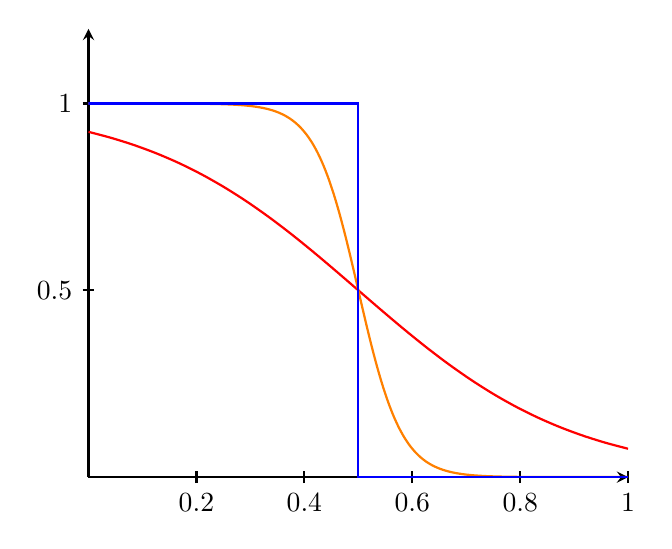
\begin{tikzpicture}
			\begin{axis}[
				domain=0:\xmax,ymax=\ymax,
				ytick={0.5,1},
				smooth,thick,
				axis lines=center,
				every tick/.style={thick},
				legend cell align=left]
				
				% Graphs
				\def\chempot{1}
				\def\n#1{1/(e^(#1*(x - \chempot+0.5)) + 1)}
				\addplot[color=red]{\n{5}};
				\addplot[color=orange,samples=100]{\n{25}};
				\addplot[const plot,color=blue] coordinates {(0,1) (\chempot-0.5,0) (\xmax,0)};
			\end{axis}
		\end{tikzpicture}
		\caption{Approximation of a non-smooth function by smooth functions. Note that the red function should be supported in $[0,1]$.}
		\label{fig:cinfty_not_complete}
	\end{figure}
	\item \textbf{Ex. 2. (Discrete Space is Incomplete)} Let $X$ be the space of real-valued sequences that only have finitely many nonzero terms. Define the norm $\norm{\{a_{n}\}} \coloneqq \sum \abs{a_{n}}$. Then $(X, \norm{\empspace})$ is incomplete. 
\end{itemize}
	
	
	
\newpage 
\section{Lecture 3: The Hahn-Banach Theorem}
\subsubsection{Addendum: Extra Applications of the Hahn-Banach Theorem}
\begin{itemize}
	\item \textbf{Exc. (Extensions of Bounded Linear Operators)} Let $X$ and $Y$ be Banach spaces, and let $M \subset X$ be a closed subspace. Let $S: M \to Y$ be a bounded linear operator. Show that: 
		\begin{enumerate}[itemsep =-2pt,label =(\arabic{*})]
			\item if $\dim{Y} < \infty$, there exists an extension of $S$ to a bounded linear operator $T: X \to Y$, 
			\item if $\dim{M} < \infty$ or $\operatorname{codim}(M) < \infty$ or $X$ is a Hilbert space, there exists a extension of $S$ to a bounded linear operator $T: X \to Y$. 
		\end{enumerate}
\end{itemize}


\newpage 
\section{Lecture 4: Weak and Strong Convergence}
\subsubsection{Key Topics:}
(1) Weak and Strong Convergence, (2) Compactness of the Unit Ball, (3) Riesz's Theorem, (4) Kakutani's Theorem 
\subsubsection{Summary:}
In this lecture, we will see a couple of different compactness results. In particular, we will study strong and weak compactness, and show that strong compactness is, in general, impossible to attain. We will see applications of these convergence types to the unit ball and reflexive spaces. 
\subsubsection{Lecture:}
\begin{itemize}
	\item \textbf{Thm. (Riesz's Theorem)} Let $X$ be a normed linear space. Then the unit ball $\{x \in X: \norm{x} \leq 1\}$ is compact if and only if $\dim(X) < \infty$.
	
	\begin{solutions}
		($\Leftarrow$) Suppose $X$ is a finite-dimensional space. In HW 2, we showed that every norm on $X$ is equivalent, and so is equivalent to the Euclidean norm. This means that the induced topology is the same as the Euclidean topology on $X$. Then since the unit sphere is closed and bounded in the Euclidean norm, by the Heine-Borel Theorem\footnote{\href{http://math.stackexchange.com/questions/4959961/heine-borel-for-finite-dimensional-normed-vector-spaces}{http://math.stackexchange.com/questions/4959961/heine-borel-for-finite-dimensional-normed-vector-spaces}}, we conclude that the unit sphere is compact. 
		
		($\Rightarrow$) Suppose that $\dim(X) = \infty$. We wish to show that the unit sphere is not compact; since $X$ is a normed (hence, metric) space, equivalence of sequential compactness and compactness implies it is sufficient to find a sequence with no convergent subsequence. In particular, we will construct a sequence $\{x_{j}\} \subseteq \{\norm{x} \leq 1\}$ so that $\norm{x_{j} - x_{k}}\geq \frac{1}{2}$ for all $j\neq k$. We proceed by induction. Choose $x_{1} \in X$ with $\norm{x_{1}} = 1$. Suppose that we have chosen $x_{1}, \ldots, x_{n}$ with $\norm{x_{j}}\leq 1$ for all $j = 1, 2,\ldots, n$, and $\norm{x_{j} - x_{k}}\geq \frac{1}{2}$ for $j \neq k$. Let $P = \operatorname{span}\{x_{1}, \ldots, x_{n}\}$. Since $P \subsetneq X$, there exists some $y_{n + 1} \in X\setminus P$ so that $\norm{y_{n + 1}}\leq \frac{1}{4}$. Let $\delta$ be the distance between $y_{n + 1}$ and $P$: 
		\begin{equation}
			\delta = \inf_{x \in P}\norm{y_{n + 1} - x} > 0. 
		\end{equation}
		In particular, there exists some $x_{\ast} \in P$ so that $\norm{y_{n + 1} - x_{\ast}} \leq (11/10)\delta$. Define the element 
		\begin{equation}
			x_{n + 1} = \frac{1}{2}\cdot \frac{y_{n + 1} - x_{\ast}}{\delta}. 
		\end{equation}
		We observe the following: 
		\begin{enumerate}[itemsep =-2pt,label = (\roman{*})]
			\item $\displaystyle \norm{x_{n + 1}} = \frac{1}{2\delta}\norm{y_{n + 1} - x_{\ast}} \leq \frac{1}{2\delta} \cdot \frac{11\delta}{10} = \frac{11}{20} < 1$. Hence, $x_{n + 1} \in \{\norm{x} \leq 1\}$. 
			\item For any $j \leq n$, 
			\begin{align}
				\begin{split}
					\norm{x_{n + 1} - x_{j}} &= \norm{\frac{y_{n + 1} - (x_{\ast} + 2\delta x_{j})}{2\delta}} \geq \frac{\delta}{2\delta} = \frac{1}{2}, 
				\end{split}
			\end{align}
			where the inequality follows from the fact that $x_{\ast} + 2\delta x_{j} \in P$. 
		\end{enumerate}
		Hence, we continue building $\{x_{j}\}$ in this way; by construction, this sequence has no convergent subsequence, which proves that the unit ball cannot be compact. 
	\end{solutions}
	\item \textbf{Rmk.} Riesz's theorem shows the problem with \textit{strong} convergence. Over the following results, we will demonstrate that \textit{weak} convergence is better for compactness. Our goal is to show that the unit ball is weakly compact in an arbitrary reflexive space. 
	\item \textbf{Def. (Weak Convergence)} Let $X$ be a normed linear space, and $X^{\ast}$ its dual space. $\{x_{n}\}_{n = 1}^{\infty} \subseteq X$ converges \textit{weakly} to $x \in X$ if for all $\ell \in X^{\ast}$, $\ell(x_{n})$ converges to $\ell(x)$. Let's recall a few results we had from last time $\ldots$
	\item \textbf{Prop. (Norm for Weak Convergence)} Let $X$ be a normed linear space, and assume $x_{n}$ converges to $x$ weakly. Then the following are true: 
	\begin{enumerate}[itemsep =-2pt,label = (\roman{*})]
		\item $\sup\limits_{n}\norm{x_{n}} < \infty$, 
		\item $\norm{x} \leq \liminf\limits_{n}\norm{x_{n}}$. 
	\end{enumerate}
	
	\begin{solutions}
		\begin{enumerate}[itemsep =-2pt,label = (\roman{*})]
			\item Uniform boundedness principle (see Lecture 5)
			\item By the Hahn-Banach Theorem, there exists a linear functional $\ell \in X^{\ast}$ with $\norm{\ell} = 1$ so that $\ell(x) = x$ (this is the second application of the HBT; see Lecture 3). This means that 
			\begin{equation}
				\norm{x} = \ell(x) = \lim_{n \to \infty}\ell(x_{n}) \leq \norm{\ell}\liminf_{n \to \infty}\norm{x_{n}} = \liminf_{n \to \infty}\norm{x_{n}}. 
			\end{equation} 
		\end{enumerate}
	\end{solutions}
	\item \textbf{Thm. (Kakutani)} Let $X$ be a normed linear space. Then $X$ is reflexive if and only if the unit ball $\{\norm{x} \leq 1\}$ is weakly compact; i.e., if and only if for any sequence $\{x_{n}\} \subseteq \{\norm{x}\leq 1\}$, there exists a subsequence $\{x_{n_{k}}\}$ and $x_{\ast} \in X$ so that $x_{n_{k}}$ converges weakly to $x_{\ast}$ as $k \to \infty$. 
	
	Remark: to prove this theorem, we will actually prove a couple of weaker results, and then use these results to attack the main theorem. Also note that the original lecture only focused on the forward direction. 
	
	\item \textbf{Thm. (Weak Kakutani)} Let $X$ be a reflexive normed linear space and $X^{\ast}$ separable. Then the unit ball $\{\norm{x_{n}} \leq 1\}$ is weakly compact. 
	
	\begin{solutions}
		Assume the hypotheses. Since $X^{\ast}$ is separable, there exists a countable dense subset $\{\ell_{n}\} \subset X^{\ast}$. Let $\{x_{n}\}$ be a subsequence of the unit ball in $X$. We will break this proof into a couple of steps. 
			\begin{quote}
				(\textbf{Step 1}) There exists a subsequence $\{x_{n_{j}}\}$ such that for all $k$, $\{\ell_{k}(x_{n_{j}})\}$ converges. 
				
				This step uses the Cantor diagonalization argument. Consider the sequence $\{\ell_{1}(x_{n_{j}})\}$. Then since this sequence is uniformly bounded, there exists a subsequence $\{x_{n_{k}}^{(1)}\}$ such that $\{\ell_{1}(x_{n_{k}}^{(1)})\}$ converges. Now consider the sequence $\{\ell_{2}(x_{n_{k}}^{(1)})\}$. Once again, this is a uniformly bounded numerical sequence, and therefore, admits a subsequence $\{x_{n_{k}}^{(2)}\}$ so that $\{\ell_{2}(x_{n_{k}}^{(2)})\}$ converges. Moreover, we also know that $\{\ell_{1}(x_{n_{k}}^{(2)})\}$ converges. Repeating this procedure inductively, construct the grid: 
					\begin{equation}
						\begin{matrix}
							x_{n_{1}}^{(1)} & x_{n_{2}}^{(1)} & x_{n_{3}}^{(1)} & \dotsm & x_{n_{k}}^{(1)} \\
							x_{n_{1}}^{(2)} & x_{n_{2}}^{(2)} & x_{n_{3}}^{(2)} & \dotsm & x_{n_{k}}^{(2)}\\
							x_{n_{1}}^{(3)} & x_{n_{2}}^{(3)} & x_{n_{3}}^{(3)} & \dotsm & x_{n_{k}}^{(3)}\\
							\vdots & \vdots & \vdots & \ddots \\
							x_{n_{1}}^{(k)} & \ldots & \ldots & \ldots &  x_{n_{k}}^{(k)} 
						\end{matrix}
					\end{equation} 
				Form a sequence by selecting all the diagonal arguments. This is the desired subsequence. 
			
			(\textbf{Step 2}) Show that this subsequence converges for \textit{all} $\ell \in X^{\ast}$.
			
			 Let $\{x_{n_{j}}\}$ be the sequence one obtains by completing Step 1. Let $\ell \in X^{\ast}$ be arbitrary Then we claim that $\{\ell(x_{n_{j}})\}$ converges: 
				\begin{align}
					\begin{split}
						\abs{\ell(x_{n_{j_{1}}}) - \ell(x_{n_{j_{2}}})} &\leq \abs{(\ell - \ell_{k})(x_{n_{j_{1}}})} + \abs{\ell_{k}(n_{j_{1}}) - \ell_{k}(n_{j_{2}})} + \abs{(\ell - \ell_{k})(x_{n_{j_{2}}})} \\
						&\leq 2 \norm{\ell - \ell_{k}} + \abs{\ell_{k}(n_{j_{1}}) - \ell_{k}(n_{j_{2}})}
					\end{split}
				\end{align}
			By density of $\{\ell_{k}\}$ in $X^{\ast}$, $\norm{\ell - \ell_{k}}$ can be made ``arbitrarily small.'' On the other hand, taking $n_{j_{1}}, n_{j_{2}} \to \infty$, we see by the claim in Step 1 that $\abs{\ell(x_{n_{j_{1}}}) - \ell(x_{n_{j_{2}}})} \to 0$. Hennce, it follows that $\{\ell(n_{j})\}$ converges. Since $\ell \in X^{\ast}$ was arbitrary, the proof concludes. 
			\end{quote}
		Now, we shall complete the proof of the theorem. Define an element $m \in X^{\ast\ast}$ as follows: for every $\ell \in X^{\ast}$, let 
			\begin{equation}
				m(\ell) \coloneqq \lim_{n_{j} \to \infty}\ell(x_{n_{j}}). 
			\end{equation}
		It is straightforward to verify that $\abs{m(\ell)} \leq \norm{\ell}$. Since $X$ is reflexive, there exists $x\in X$ such that $m(\ell) = \ell(x)$. In other words, 
			\begin{equation}
				\lim_{j \to \infty}\ell(x_{n_{j}}) =\ell(x), \qquad \forall \ell \in X^{\ast}. 
			\end{equation}
		Hence, the unit ball is weakly compact. 
	\end{solutions}
	\item \textbf{Lem. (Separability of $X$)} Let $X$ be a normed linear space, and $X^{\ast}$ its dual. If $X^{\ast}$ is separable, then $X$ is separable. This was proven in HW 2. 
	
	\item \textbf{Lem. (Reflexivity of Closed Subspaces)} If $X$ is reflexive, then any closed subspace $Y \subset X$ is reflexive. 
	
	\begin{solutions}
		Our goal is to show that given $m \in Y^{\ast\ast}$, there exists some $y \in Y$ so that for all $\ell \in Y^{\ast}$, $m(\ell) = \ell(y)$. Note that the map $\ell \mapsto \ell|_{Y}$ defines a map from $X^{\ast}$ to $Y^{\ast}$. So consider the map $X^{\ast} \ni \ell \mapsto m(\ell|_{Y})$, which defines an element in $X^{\ast}$. Since $X$ is reflexive, there exists an $x_{0} \in X$ such that $m(\ell|_{Y}) = \ell(x_{0})$ for all $\ell \in X^{\ast}$. We must show the following: 
			\begin{enumerate}[itemsep =-2pt,label= (\arabic{*})]
				\item $x_{0} \in Y$;
				\item for all $\ti{\ell} \in Y^{\ast}$, $m(\ti{\ell}) = \ti{\ell}(x_{0})$. 
			\end{enumerate}
		Let us prove each claim individually. 
			\begin{enumerate}[itemsep =-2pt,label = (\arabic{*})]
				\item Assume to the contrary that $x_{0}\notin Y$. Then there exists some $\ell \in X^{\ast}$ so that $\ell|_{Y} = 0$ and $\ell(x_{0}) \neq 0$ (by Hahn-Banach). But this is impossible by the line defining $x_{0}$. Hence, $x_{0}\in Y$. 
				\item Consider $\ti{\ell} \in Y^{\ast}$. Then by Hahn-Banach, we can produce some $\ell \in X^{\ast}$ such that $\ell|_{Y} = \ti{\ell}$. Hence, $m(\ti{\ell}) = m(\ell|_{Y}) = \ell(x) = \ti{\ell}(x_{0})$. 
			\end{enumerate}
		Hence, the proof concludes. 
	\end{solutions} 
	
	\item \textbf{Prf. (Kakutani)} Now we will use the two preceding lemmas and the weak Kakutani theorem to prove the main theorem. Let $\{x_{n}\}_{n= 1}^{\infty}$ be a subsequence of the closed unit ball in $X$. Let $Y = \overline{\operatorname{span}\{x_{n}\}}$. Since $Y$ is a closed subspace of $X$ and $X$ is reflexive, $Y$ is reflexive. On the other hand, since every subspace of a separable metric space is separable, $Y = (Y^{\ast})^{\ast}$ is separable. Hence, in particular, $Y^{\ast}$ is separable by the first lemma. By the weak Kakutani theorem, $\{\norm{x} \leq 1\} \cap Y$ is weakly compact. Hence, there exists a subsequence $\{x_{n_{k}}\}$ so that for all $\ell \in Y^{\ast}$, $\ell(x_{n_{k}}) \to \ell(x_{\ast})$. Since for any $\ell \in X^{\ast}$, $\ell|_{Y} \in Y^{\ast}$, we conclude that 
		\begin{equation}
			\ell(x_{n_{k}}) = \ell|_{Y}(x_{n_{k}}) \longrightarrow \ell|_{Y}(x_{\ast}) = \ell(x_{\ast}). 
		\end{equation} 
	This concludes the proof. 
\end{itemize}
\end{document}